\section{Methodology}\label{sec:methodology}

\subsection{Approach}\label{subsec:approach}

This project follows a prototype-driven methodology, which involves iterative development and testing of prototypes to refine the final product.
The methodology consists of the following phases:

\begin{itemize}
    \item \textbf{Web crawling and data collection:} The initial phase involves crawling the set of selected websites to store each page's HTML content for later use.
    This is done using a web crawler that systematically navigates through the websites and collects the necessary data.
    This phase always involves the use of a queue to manage the URLs to be crawled, ensuring that the crawler can efficiently handle large numbers of pages, while minimizing the number of duplicate pages crawled.

    \item \textbf{Data annotation:} A subset of the collected pages are then manually labelled to create a suitable machine learning model for future classification, information extraction, and product matching tasks.
    The pages were labelled based on the following characteristics:
    \begin{itemize}
        \item \textbf{Page type:} Each page is classified as either a product page, a product list page, an error page, or other.
        \item \textbf{Product information:} For product pages, relevant product information such as product name, price, and description is extracted and stored in a structured format.
    \end{itemize}

    \item \textbf{Boilerplate removal:} Since the collected HTML pages contain a significant amount of boilerplate content (e.g., navigation menus, advertisements, and other non-essential elements), a boilerplate removal step is performed to extract the main content of each page.
    This is done in order to minimize the amount of noise in the data and improve the accuracy of subsequent machine learning models, as well as reduce the number of tokens to be processed, which can significantly improve the performance  and resource usage of the models.

    \item \textbf{Page classification:} A machine learning model is trained to classify the pages into the two main categories: product pages and non-product pages.
    This model is trained using the manually labelled data from the previous phase, and is then used to automatically classify the remaining pages in the dataset.

    \item \textbf{Information extraction:} For the pages classified as product pages, a machine learning model is trained to extract relevant product information such as product name, price, and description.
    This model is also trained using the manually labelled data from the data annotation phase, and is then used to automatically extract product information from the remaining product pages in the dataset.

    \item \textbf{Product matching:} Finally, a product matching model is trained to identify and link identical products across different websites.
    This model is trained using the extracted product information from the previous phase, and is then used to automatically match products across different websites in the dataset.
\end{itemize}

Each phase of the methodology is iterative, with the results of each phase informing the next phase.

Finally, the results from all the phases are combined to create a \textbf{proof-of-concept (PoC) system}, which is a web-based application that allows users to search for products, analyze their price history, and compare prices across different websites.

Figure~\ref{fig:page_lifecycle} illustrates the expected happy path that would be followed by a page in the project, going through each phase from crawling to its appearance in the PoC application.

\begin{figure}[h]
    \centering
    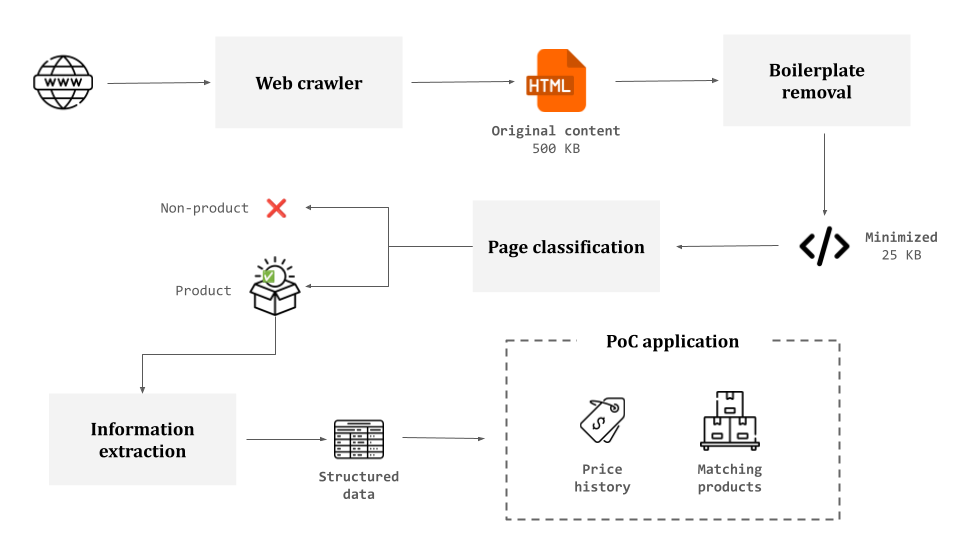
\includegraphics[width=0.8\textwidth]{images/page_lifecycle}~\caption{Lifecycle of a page}
    \label{fig:page_lifecycle}
\end{figure}

\subsection{Evaluation}\label{subsec:evaluation}

Each phase of the project is evaluated using different sets of qualitative metrics to assess the performance and effectiveness of the models and methods used.
The evaluation metrics used for each phase are as follows.

\begin{table}[h]
    \centering
    \small
    \renewcommand{\arraystretch}{1.4}
    \begin{tabularx}{\textwidth}{p{4cm} X}
        \toprule
        \textbf{Phase} & \textbf{Evaluation metrics} \\
        \midrule
        Web crawler & \begin{minipage}[t]{\linewidth}\raggedright \textbullet{} Number of pages crawled in 24 hours\par \textbullet{} Number of uncrawled pages in a 72-hour window\par \textbullet{} Average daily cost in USD\end{minipage} \\
        \midrule
        Data annotation & N/A \\
        \midrule
        Boilerplate removal & \begin{minipage}[t]{\linewidth}\raggedright \textbullet{} Average page size reduction (as a percentage of original content)\par \textbullet{} Average time and cost required to minimize 5000 pages\end{minipage} \\
        \midrule
        Page classification & \begin{minipage}[t]{\linewidth}\raggedright \textbullet{} F1-score of the classification model on the validation dataset\par \textbullet{} Time and cost required to train and tune the model\par \textbullet{} Average time and cost required to classify 5000 pages\end{minipage} \\
        \midrule
        Information extraction & \begin{minipage}[t]{\linewidth}\raggedright \textbullet{} Weighted accuracy of the model in successfully extracting the product title and price from the validation dataset\par \textbullet{} Time and cost required to train and tune the model\par \textbullet{} Average time and cost required to extract information from 5000 pages\end{minipage} \\
        \midrule
        Product matching & \begin{minipage}[t]{\linewidth}\raggedright \textbullet{} Time and cost required to train and tune the model\par \textbullet{} F1-score of the model in product matching on the validation dataset\end{minipage} \\
        \midrule
        PoC application & \begin{minipage}[t]{\linewidth}\raggedright \textbullet{} Average time (in ms) taken to retrieve the price history of a single product\par \textbullet{} Average time (in ms) taken to match similar products for a specific product\end{minipage} \\
        \bottomrule
    \end{tabularx}
    \caption{Evaluation metrics used for each phase}
    \label{tab:evaluation_metrics}
\end{table}